% !TEX root = thesis.tex
\renewcommand{\thefigure}{2.1}
\begin{figure*}
  \centering
  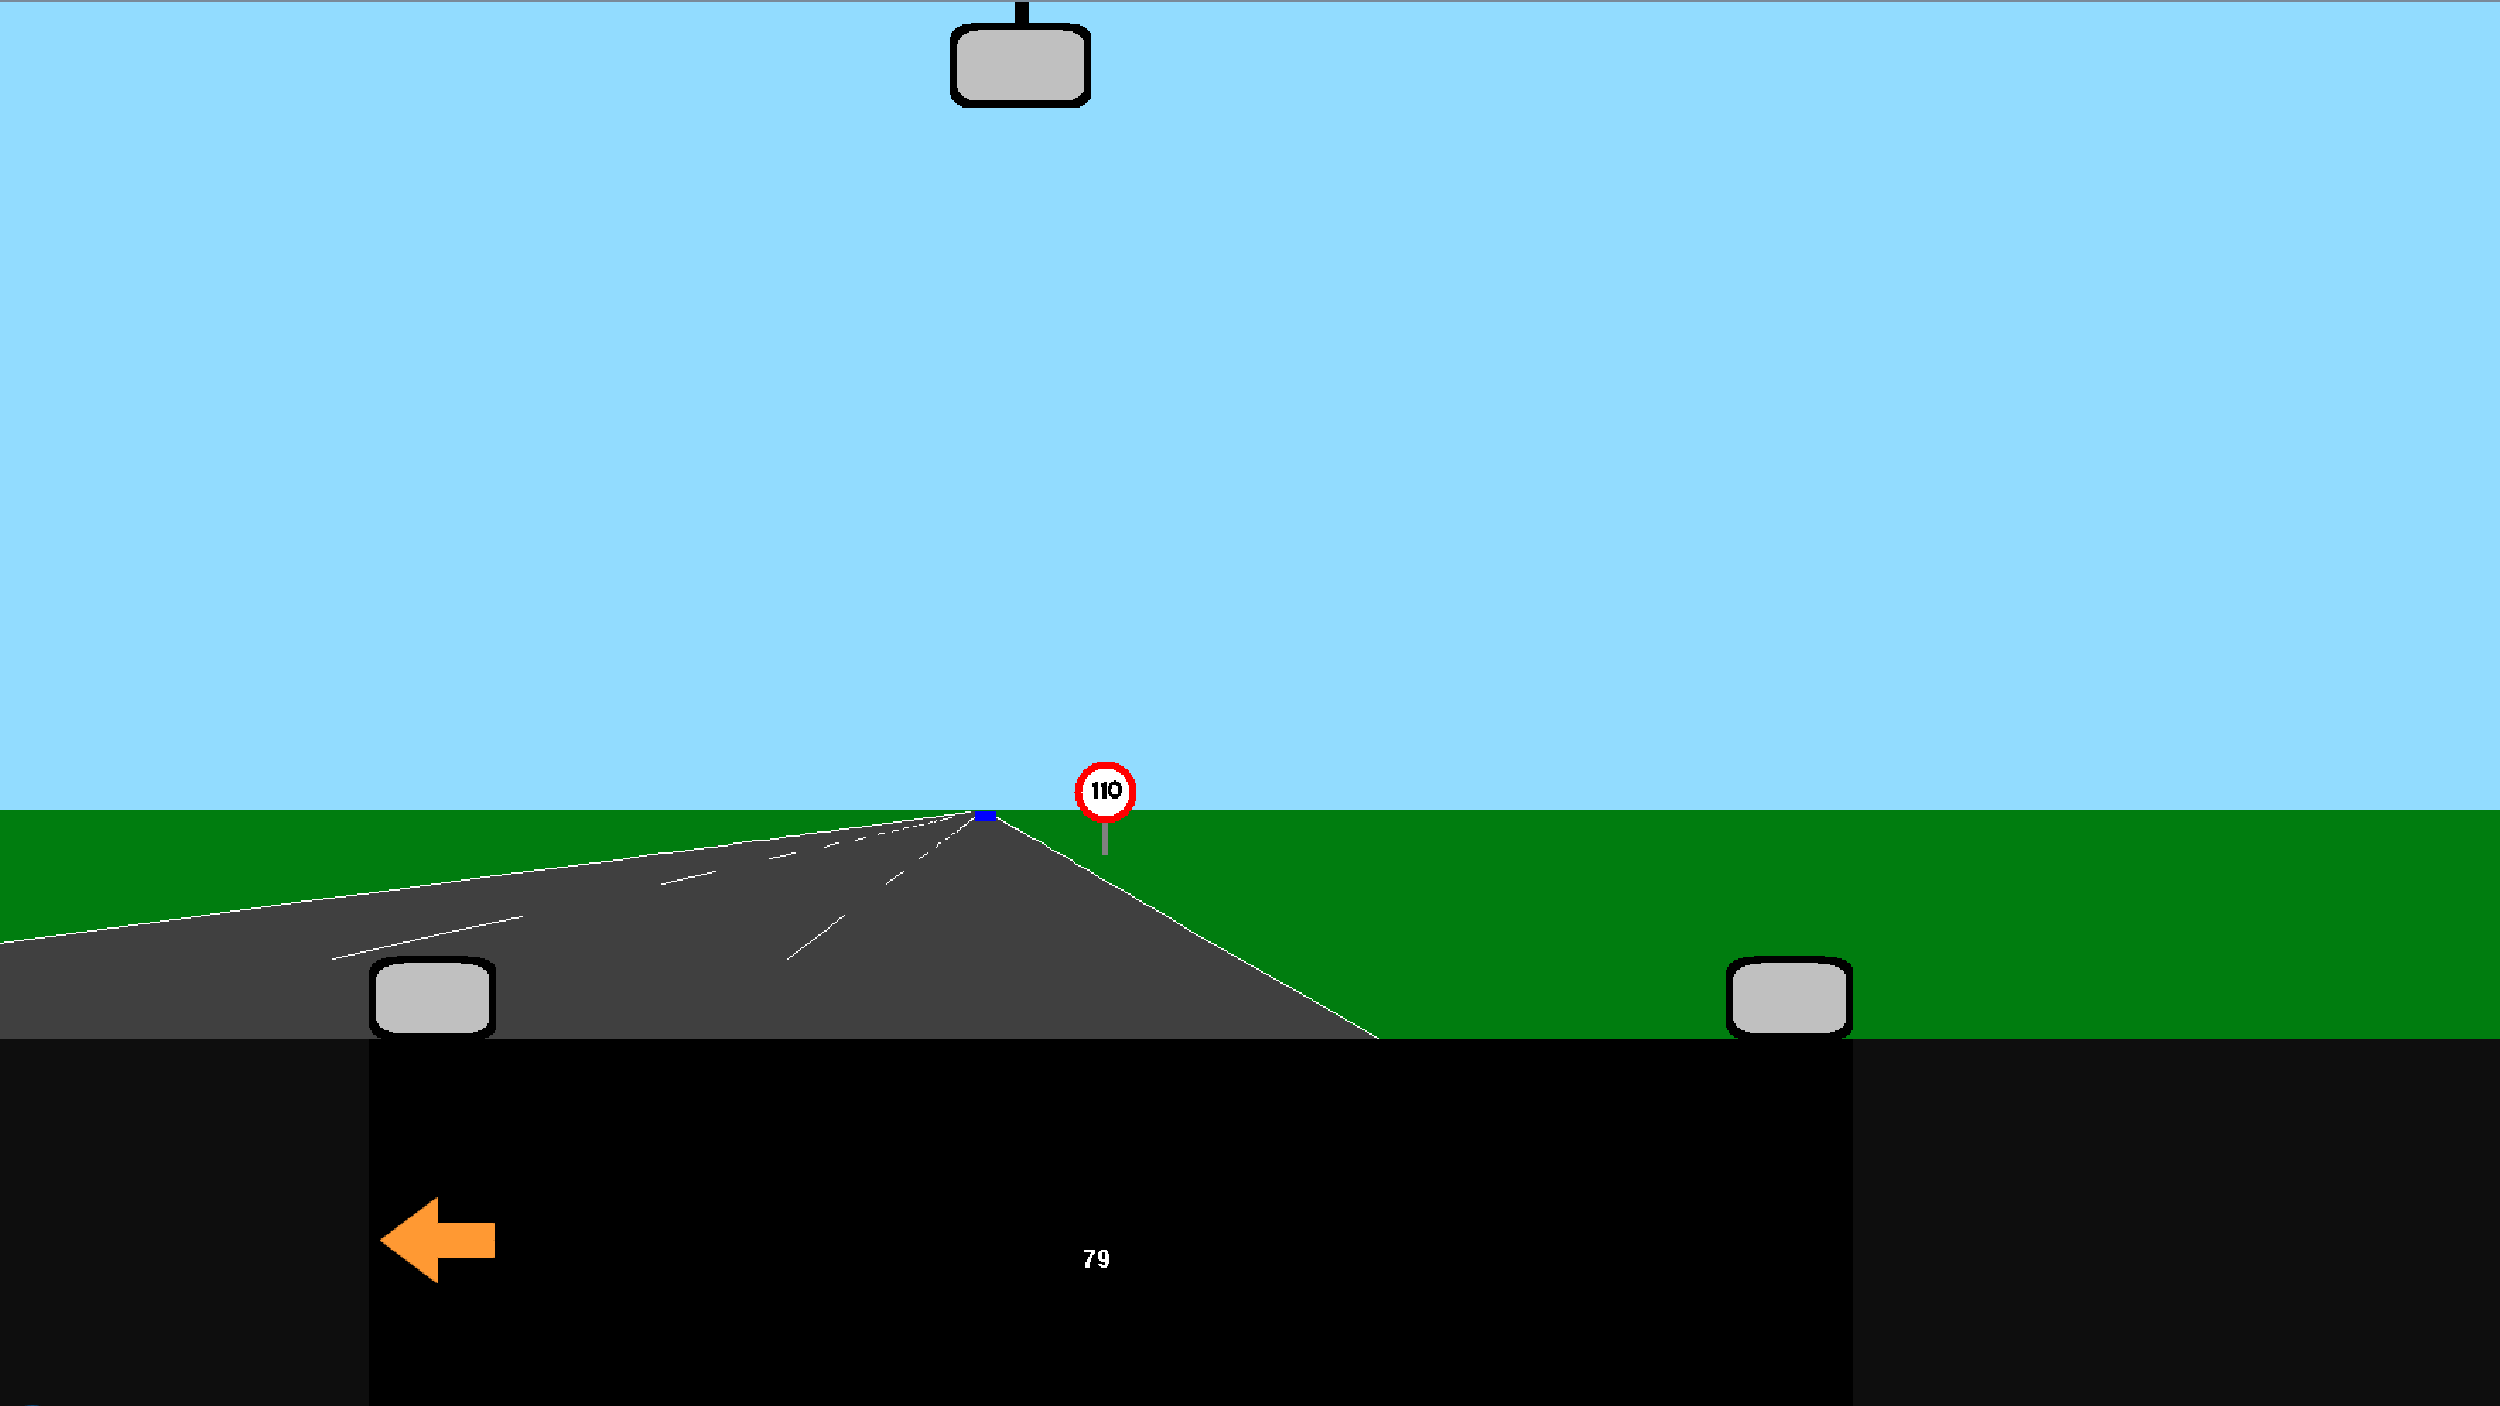
\includegraphics[width=\textwidth]{images/screenshot_noncon_blinker.pdf}
  \caption{The driving simulation for the non-construction condition.
  The orange arrow on the left of the dashboard is the indicator that blinks three times once the participant presses the indicator.
  The number at the center of the dashboard shows the current driving speed. 
  At the top and on both sides of the screen are mirrors in which the participant can see the autocar when it is behind them.}
  \label{fig:screenshot_noncon}
\end{figure*}

\section{Methods}\label{sec:methods}
\subsection{Participants}
A total of 38 volunteers (23 male, 12 female, 3 other/undisclosed) aged 20--36 (\(M = 23.1 \pm 3.0\)) participated in this experiment. 
They all had a driver's license, on average for 4.5 years (\(\pm\ 3.1\)).
All participants signed an informed consent form prior to the experiment and were compensated 12 euros for their participation.

\subsection{Materials}
% equipment
Participants interacted with the driving simulation using a steering wheel with indicators and a throttle and brake pedal (Driving Force GT, Logitech, Lausanne, Switzerland). 
The steering wheel was secured to the table in front of the screen and remained in the same location for all participants. 
The pedals were placed on the floor such that participants could move it closer or further depending on their level of comfort. 
An eye-tracking camera (EyeLink Portable Duo, SR Research, Missisauga, Canada), placed between the screen and the steering wheel, was used to continuously record the eye movements and pupil size of participants. 
The method of tracking that we employed was remote tracking using a target sticker on the participant's forehead.
This method was chosen because stabilizing the head using a head rest was not feasible considering the set-up with the steering wheel.

% environment
The simulated environment of the experiment consisted of a straight three-lane highway, as shown in Figure~\ref{fig:screenshot_noncon}.
The features of the environment were minimal. 
Either side of the road was coloured green, signifying grass. 
Traffic consisted of a single other car on the highway, referred to as the \textit{autocar} and represented by a blue rectangle.
The autocar would stick to traffic rules such as overtaking from the left, staying on the right lane as much as possible, and following the current speed limit. 

\renewcommand{\thefigure}{2.2}
\begin{figure*}
  \centering
  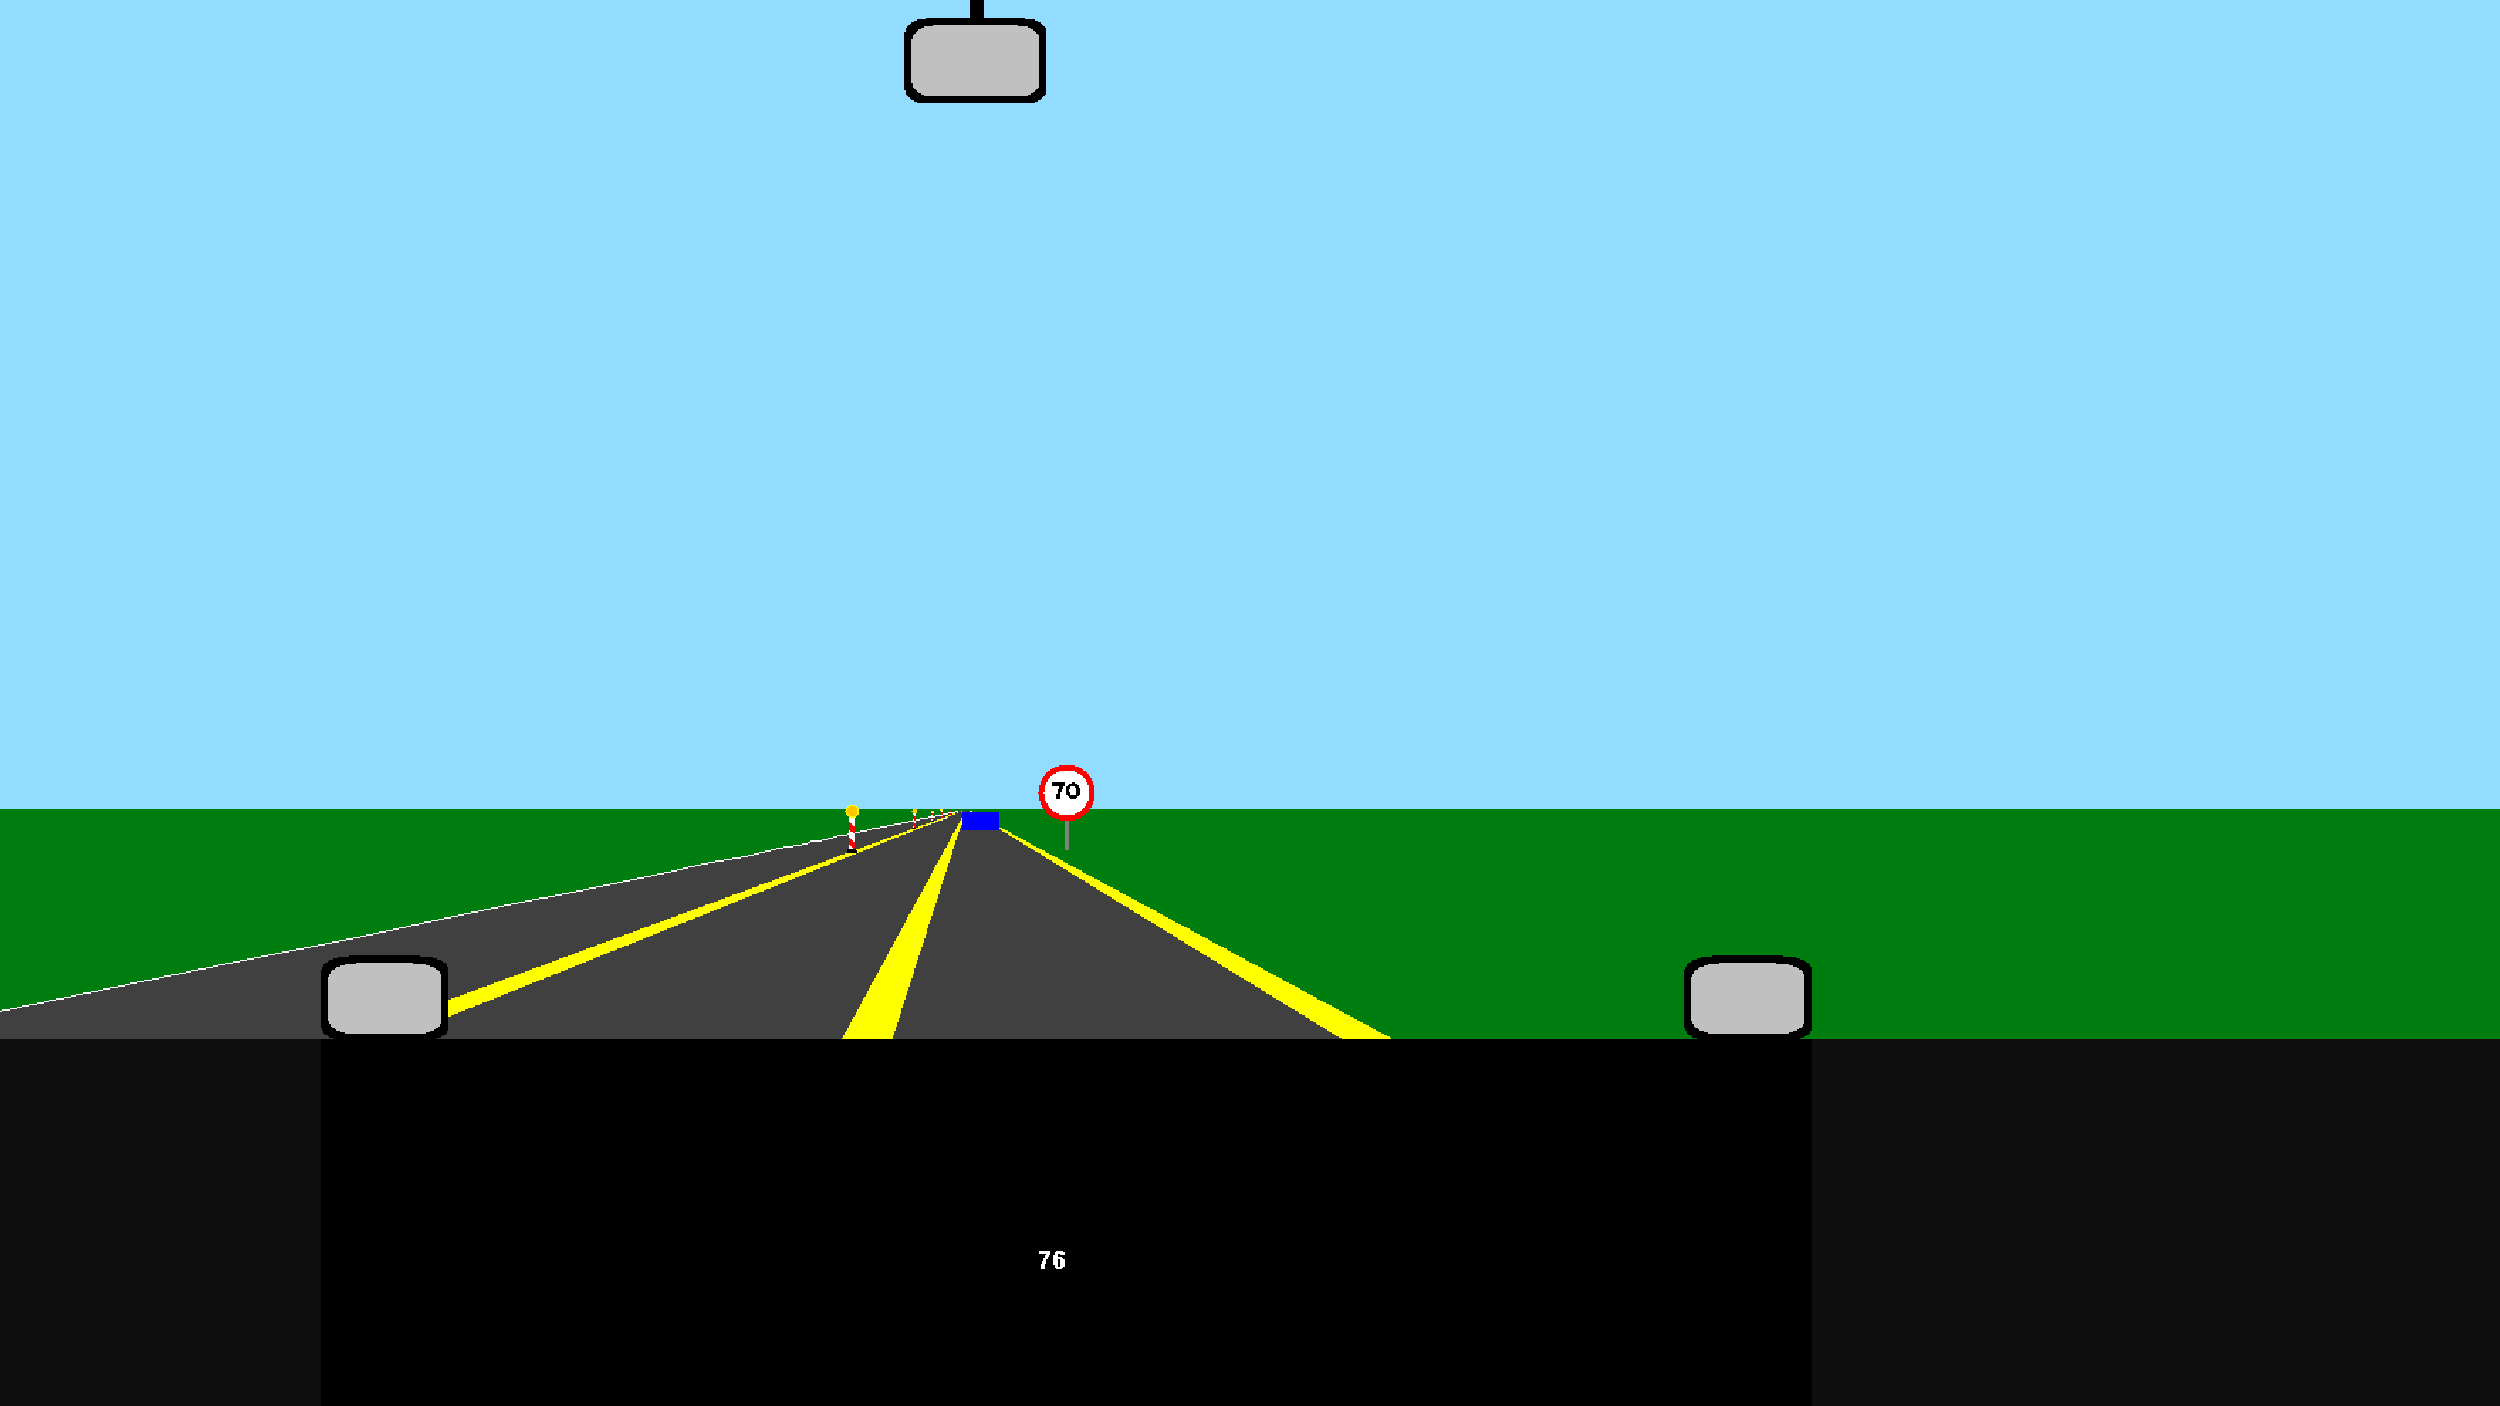
\includegraphics[width=\textwidth]{images/screenshot_con.pdf}
  \caption{The driving simulation for the construction condition. 
  The leftmost lane is closed off by a row of pylons and the remaining lanes are more narrow than in the non-construction condition. 
  The autocar can be seen next to the speed sign.}
  \label{fig:screenshot_con}
\end{figure*}

% car itself
The bottom of the screen was filled by a black dashboard. 
At the center of the dashboard the current speed of the car was shown as an integer.
When the left or right indicators were pressed, they would appear on the dashboard in the respective sides as orange blinking arrows. 
The simulation had three rear-view mirrors: one on the top, one on the left, and one on the right. 
The autocar was visible in the corresponding mirrors depending on the distance from the car. 

% construction
In the construction condition the leftmost lane is closed off by a row of pylons as shown in Figure~\ref{fig:screenshot_con}. 
The lanes were separated by a full yellow line and were narrower than in the non-construction condition. 

% speed signs
Speed signs that passed were identical to general speed signs in The Netherlands: black digits enclosed by a red circle. 

% n-back task
The \nback task that participants performed during driving is illustrated best by an example from \citet{Unni2017} as shown in Figure~\ref{fig:nback_scheme}, which they explain as follows.
In this scenario the participant is about to pass the 80 km/h speed sign and the previous four speed signs were as shown in the schematic. 
For the corresponding \textit{n}-back task, participants had to memorize the last \textit{n} speed signs and drive at the \textit{n}th speed sign which occurred previously.
For example, at 1-back, the participant’s target speed is the previous sign (140 km/h) and has to keep the current speed sign in memory (80 km/h).

\renewcommand{\thefigure}{2.3}
\begin{figure}
  \centering
  \includegraphics[width=7cm]{images/nback_Scheunemann.pdf}
  \caption{Example of \textit{n}-back experimental paradigm to manipulate working memory load (from \citealp{Unni2017}).}
  \label{fig:nback_scheme}
\end{figure}

A trial consisted of the participants performing the speed-regulating task for nine speed signs. 
The speeds shown on the signs were randomized in the range 40--120 km/h in steps of 10 km/h.
The signs appeared at intervals of 20 seconds, with the first speed sign being passed at 5 seconds.
For \nback tasks with \(n \geq 1\) there was a so-called ``build-up phase'' of \(n\) speed signs during which the participant did not need to regulate their speed yet. 
For example, for \(n = 4\), the build-up phase would be the first four speed signs. 
They would then have to start the speed-regulating task at the fifth speed sign.
Because of the build-up phase, the \nback trials differed in number of speed signs shown and therefore in duration.
It is important to note here that the build-up phase is excluded from data analysis since it is not considered a part of the \nback task. 

\subsection{Experimental Procedure}
There are 10 unique combinations of \nback level and construction condition.
Each of these combinations was performed twice, resulting in a total number of 20 trials.
These were divided into two blocks of 10 trials with a short break in between.

The order of the trials was determined pseudorandomly with a few conditions. 
Firstly, no \nback level could appear twice in a row. 
Secondly, the construction/non-construction conditions were alternated from trial to trial. 
Thirdly, the order of the trials in the first block was reversed to form the order of trials in the second block.
These constraints on the randomization were incorporated with the aim of avoiding habituation effects for the memory task and the visuospatial demands.

Prior to performing the experiment the participant was given instructions about the driving and the memory task. 
They then performed a practice round (one 2-back trial with no construction and a total of 5 speed signs) to get accustomed to the task, the simulation and the steering wheel. 
Next, the eye-tracker was calibrated, which required the participant to follow a target around the computer screen with their eyes. 
This procedure was repeated twice: once to calibrate and once to validate whether that calibration was accurate. 
If validation was inaccurate, calibration was repeated.

After calibration, the experiment began. 
Every trial (excluding the very first one) was preceded by an eye-tracking drift correction. 
This required the participant to look at a target at the center of the screen. 
If the measured eye position deviated too far from the position of the target, calibration was performed again. 
Otherwise the deviation was automatically taken into account with recording of the eye position.
Following drift correction, a pop-up message appeared telling the participant which \nback task they were about to perform.
The percentage of total trials they had already completed was also shown in the message. 
The participant could then start the trial by pressing an OK button on the steering wheel.
Unlike in the experiment by \citeauthor{Scheunemann2019}, we did not include warning messages telling participants to change their speed when it was incorrect.
We did this to prevent participants guessing the correct speed.

\subsection{Data collection}
A number of different variables pertaining to driving behavior were recorded at a rate of 200 Hz. 
The use of the accelerator and brake pedals was recorded as numbers ranging from 0 (not pressed) to 1 (fully pressed). 
The angle of the steering wheel was recorded as a number ranging from -1 (left) to 1 (right).
In order to measure lane centering, the position and orientation of the participant's car were recorded. 
Finally, the speed of the participant's car was recorded along with the occurring speed signs to calculate \nback task performance. 

The eye-tracker recorded a number of raw variables at a rate of 500 Hz, two of which are relevant for the current study.
Eye positions were measured in \(x\) and \(y\) coordinates relative to the PC monitor (\(1920 \times 1080\) px).
Pupil size was measured in terms of diameter in arbitrary units.
The eye-tracker recorded only one eye (specifically the left) as this is most common in eye-tracking experiments \citep{Hutton2019}.

\subsection{Data analysis}
All analyses were conducted using the R programming language \citep{R}.

The raw eye-tracking data were sorted into fixations, saccades and blinks using the \texttt{eyelinker} R package \citep{eyelinker}.
Only the fixations were used for data analysis as these are the most reliable measurements of both pupil size and fixation location.

To properly compare pupil size within and between participants, baseline correction is required. 
According to \citet{Mathot2018} baseline correction increases statistical power by accounting for random fluctuations in pupil size over the course of an experiment.
To this end, the baseline pupil size is recalculated for each new trial.
As a baseline period we chose the time period between the start of the trial and the appearance of the first speed sign.
The mean pupil size during this 5 second interval was used to correct the pupil sizes of the trial.
The specific method of baseline correction that we used is subtractive baseline correction (\(corrected\ pupil\ size = pupil\ size - baseline\)) 
as \citet{Mathot2018} prefer it over divisive baseline correction (\(corrected\ pupil\ size = pupil\ size / baseline\)).

In order to analyze fixations on the speedometer it must be defined as an area of interest (AOI).
The bounds of this AOI could not be universally defined since the measurement of eye-positions shifted between and within participants.
For this reason we manually determined the borders of the AOI for each participant; in other words, we determined what ``counts as'' a fixation on the speedometer.
Fixations on the speedometer will be expressed as a percentage of the total number of fixations during that trial.

We will focus on three measures relating to the two variables of interest. 
Pupil size will be examined both between and within trials.
These two temporal contexts will provide a detailed image of how a participant's pupil size changes over time.
Fixations on the speedometer will be examined between trials. 
In order to test the significance of the results we will use a two-way ANOVA with repeated measures, with \nback level and construction/non-construction as independent variables.